\documentclass[11pt, a4paper]{article}
\usepackage{pdfpages}
\usepackage{parallel}
\usepackage[T2A]{fontenc}
%\usepackage{ucs}
\usepackage[utf8]{inputenc}
\usepackage[english,russian]{babel}
\usepackage{hyperref}
\usepackage{rotating}
\usepackage[inner=2cm,top=1.8cm,outer=2cm,bottom=2.3cm,nohead]{geometry}
%\usepackage{listings}
\usepackage{graphicx}
\usepackage{wrapfig}
\usepackage{longtable}
\usepackage{indentfirst}
\usepackage{array}
\usepackage{tikzsymbols}
\usepackage{soul}
\usepackage[ruled,vlined]{algorithm2e}
\usepackage{qrcode}
\counterwithout{figure}{section} 

\usepackage{url}
\makeatletter
\g@addto@macro{\UrlBreaks}{\UrlOrds}
\makeatother

\newcolumntype{P}[1]{>{\raggedright\arraybackslash}p{#1}}
\frenchspacing
%\usepackage{fixltx2e} %text sub- and superscripts
\usepackage{icomma} % коскі ў матэматычным рэжыме
%\PreloadUnicodePage{4}

\newcommand{\longpage}{\enlargethispage{\baselineskip}}
\newcommand{\shortpage}{\enlargethispage{-\baselineskip}}

\def\switchlang#1{\expandafter\csname switchlang#1\endcsname}
\def\switchlangbe{
\let\saverefname=\refname%
\def\refname{Літаратура}%
\def\figurename{Іл.}%
}
\def\switchlangru{
\let\saverefname=\refname%
\let\savefigurename=\figurename%
\def\refname{Литература}%
\def\figurename{Рис.}%
}
\def\switchlangen{
\let\saverefname=\refname%
\def\refname{References}%
\def\figurename{Fig.}%
}

\hyphenation{admi-ni-stra-tive}
\hyphenation{ex-pe-ri-ence}
\hyphenation{fle-xi-bi-li-ty}
\hyphenation{Py-thon}
\hyphenation{ma-the-ma-ti-cal}
\hyphenation{re-ported}
\hyphenation{imp-le-menta-tions}
\hyphenation{pro-vides}
\hyphenation{en-gi-neering}
\hyphenation{com-pa-ti-bi-li-ty}
\hyphenation{im-pos-sible}
\hyphenation{desk-top}
\hyphenation{elec-tro-nic}
\hyphenation{com-pa-ny}
\hyphenation{de-ve-lop-ment}
\hyphenation{de-ve-loping}
\hyphenation{de-ve-lop}
\hyphenation{da-ta-ba-se}
\hyphenation{plat-forms}
\hyphenation{or-ga-ni-za-tion}
\hyphenation{pro-gramming}
\hyphenation{in-stru-ments}
\hyphenation{Li-nux}
\hyphenation{sour-ce}
\hyphenation{en-vi-ron-ment}
\hyphenation{Te-le-pathy}
\hyphenation{Li-nux-ov-ka}
\hyphenation{Open-BSD}
\hyphenation{Free-BSD}
\hyphenation{men-ti-on-ed}
\hyphenation{app-li-ca-tion}

\def\progref!#1!{\texttt{#1}}
\renewcommand{\arraystretch}{2} %Іначай формулы ў матрыцы зліпаюцца з лініямі
\usepackage{array}

\def\interview #1 (#2), #3, #4, #5\par{

\section[#1, #3, #4]{#1 -- #3, #4}
\def\qname{LVEE}
\def\aname{#1}
\def\q ##1\par{{\noindent \bf \qname: ##1 }\par}
\def\a{{\noindent \bf \aname: } \def\qname{L}\def\aname{#2}}
}

\def\interview* #1 (#2), #3, #4, #5\par{

\section*{#1\\{\small\rm #3, #4. #5}}
\ifx\ParallelWhichBox\undefined%
    \addcontentsline{toc}{section}{#1, #3, #4}%
\else%
\ifnum\ParallelWhichBox=0%
    \addcontentsline{toc}{section}{#1, #3, #4}%
\fi\fi%

\def\qname{LVEE}
\def\aname{#1}
\def\q ##1\par{{\noindent \bf \qname: ##1 }\par}
\def\a{{\noindent \bf \aname: } \def\qname{L}\def\aname{#2}}
}

\newcommand{\interviewfooter}[1]{
\vskip 1em
\noindent \textit{#1}
}

\AtEndDocument{\vfill\centering \qrcode{https://github.com/fiowro/mouses/blob/main/\jobname.pdf}}

\switchlang{en}
\begin{document}

\title{1981 -- Xerox Alto Optical Mouse}
\date{}
\maketitle
\selectlanguage{english}

In March 1973, Xerox Corporation announced the Xerox Alto computer, considered the first workstation (or personal computer), as well as the first computer with a graphical user interface \cite{wiki}. The workstation also came with the first mass-produced mouse in the history of computers, the Xerox Alto Mouse (fig. \ref{fig:XeroxAltoPic}). The original mouse based on two wheels was in several years upgraded and started to use a ball. But still, those mice weren't too reliable according to the quotes given in \cite{mouses}: they picked up dirt, quickly became gummed, and no longer controlled the cursor. Alto user had to unplug the mouse when that happened, put it into the ``Dead Mice''  box, and grab a cleaned mouse from the ``Clean Mice'' box. And the price of such a mouse was more than \$400.

The work for a completely optical mouse has been started near 1980 to solve two problems: to get higher reliability (because of no moving parts except the button switches), and much cheaper price (due to the one-chip design). The result of this effort was the last generation of the Alto mice -- Xerox Alto optical mouse, brought into life in 1981 \cite{vlsi81}. The mouse proved to be very successful compared to its mechanical predecessor, so its design was soon adopted for Xerox Star computers and later even for some of the company's copiers \cite{mouses}.

\begin{figure}[h]
    \centering
    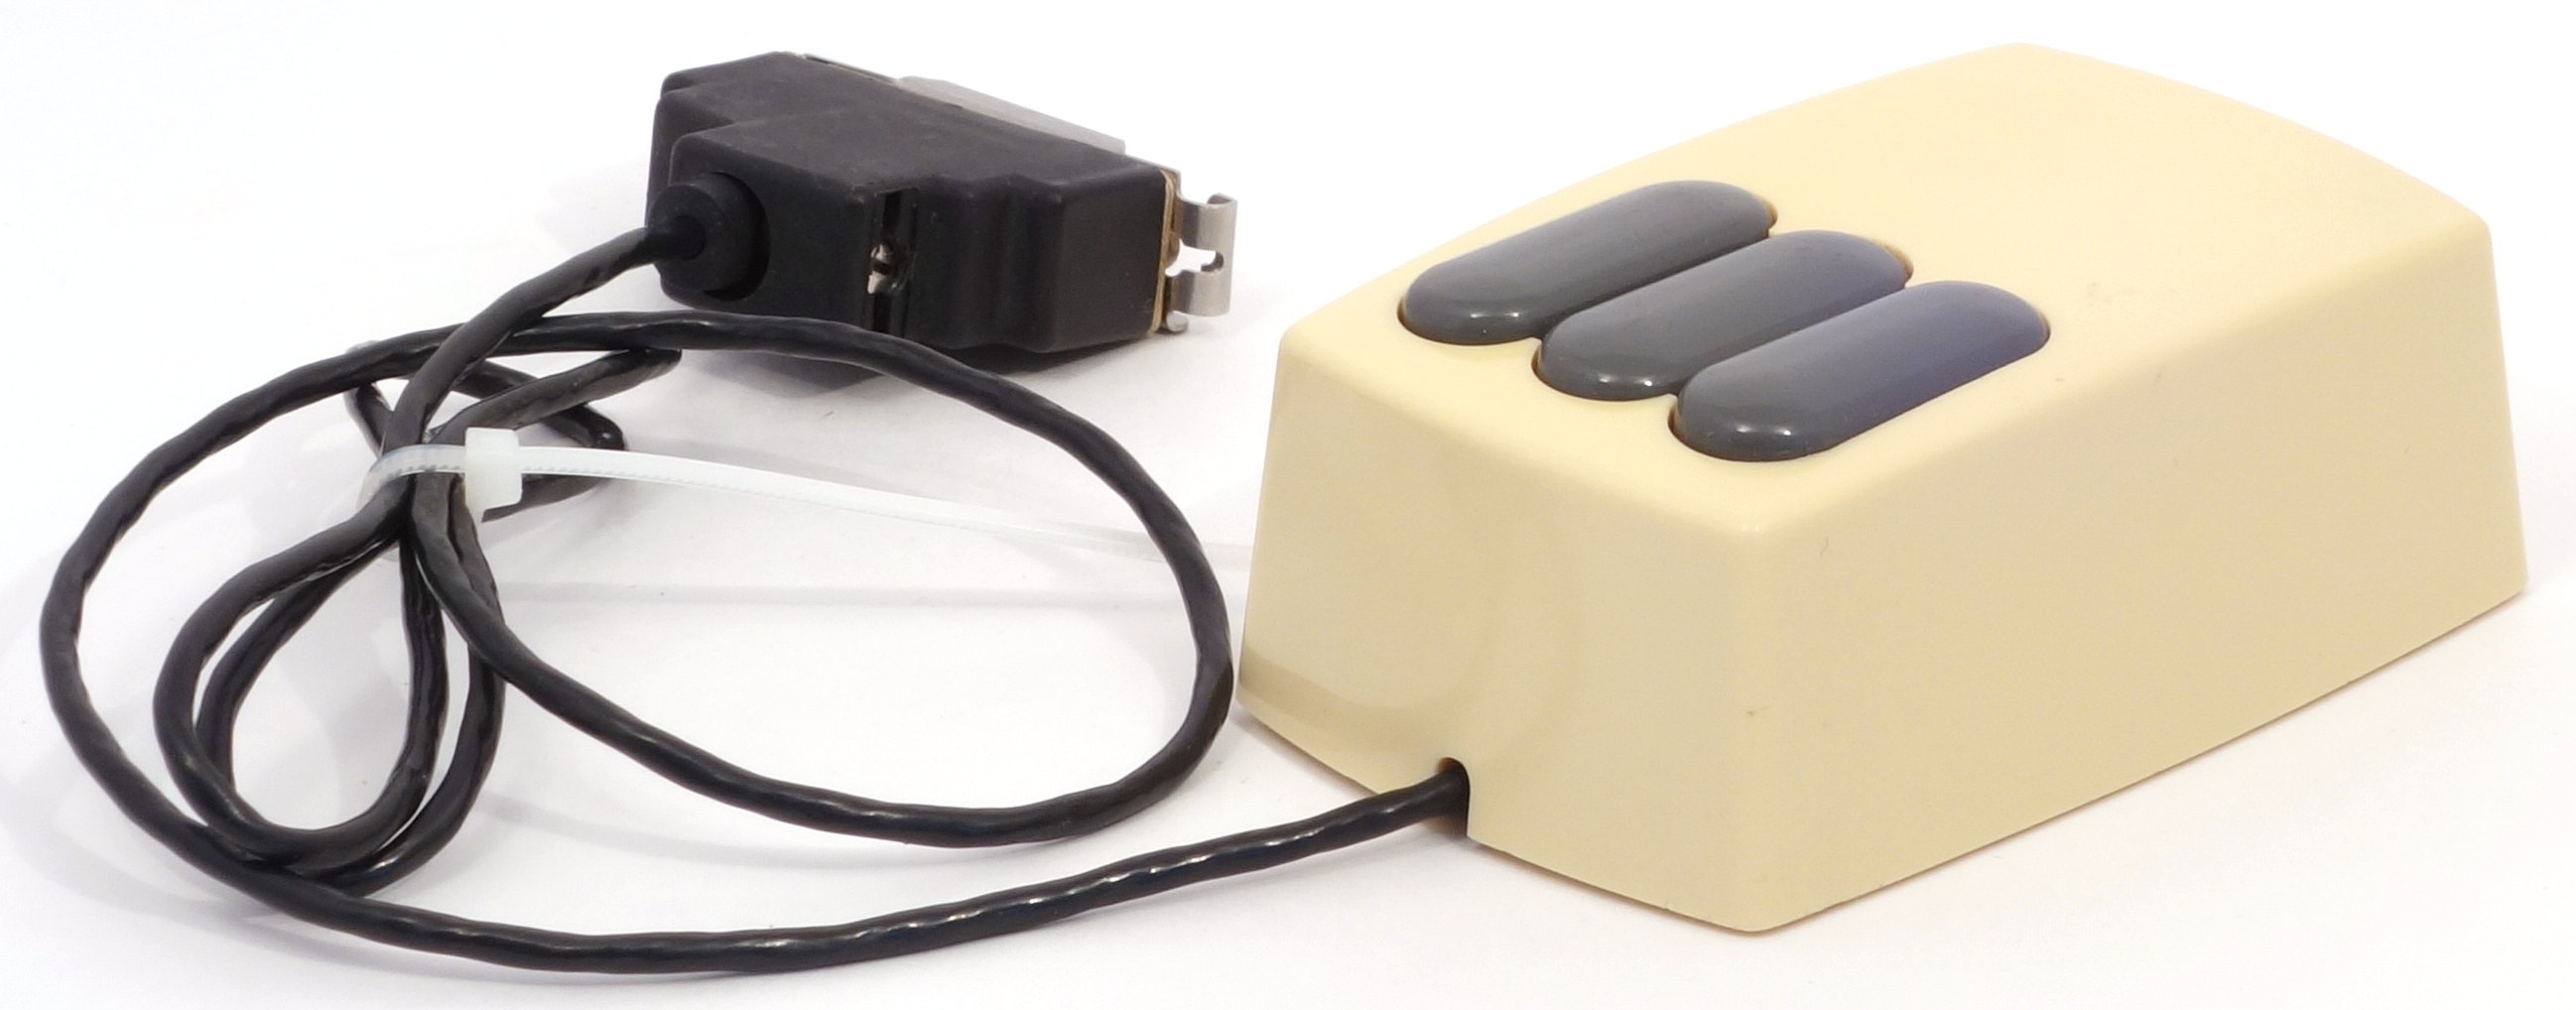
\includegraphics[scale=0.7]{1981_xerox_alto_mouse/pic_30.jpg}
    \caption{Xerox Alto Optical Mouse}
    \label{fig:XeroxAltoPic}
\end{figure}

The Xerox Alto optical mouse is housed in the same case as its mechanical version \cite{vlsi82}, and has the same color scheme. The case, made of (originally) cream-colored plastic, glossy in this mouse revision, is an almost perfect parallelepiped: it widens slightly toward the bottom and has convex sides to reduce the association with a ``box''. On the upper side of the case are three large, oblong, rounded buttons that meet at the edges, visually forming one solid block (Fig. \ref{XeroxAltoTopAndBottom}). Xerox software documentation called these buttons ``red'', ``yellow'', and ``blue''. However, in all cases (except for the earliest mouse modification with wheels and transversely oriented buttons \cite{vlsi81}), all three buttons were made of black (later, dark gray) plastic. It is likely that the myth that using one- and two-button mice was easier compared to a three-button one comes out of the confusion this unfortunate color coding caused among users.

\begin{figure}[h]
    \centering
    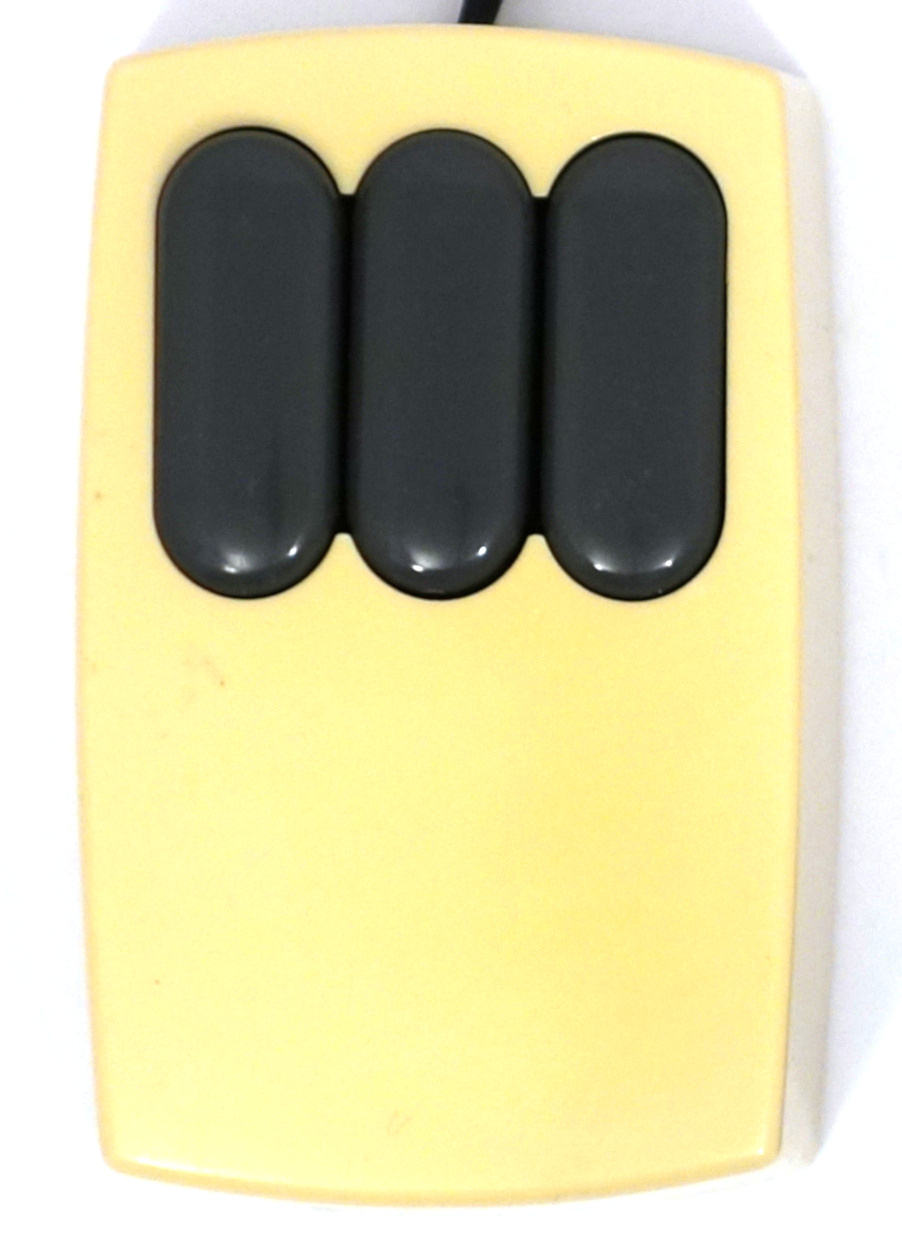
\includegraphics[scale=0.5]{1981_xerox_alto_mouse/top_30.jpg}
    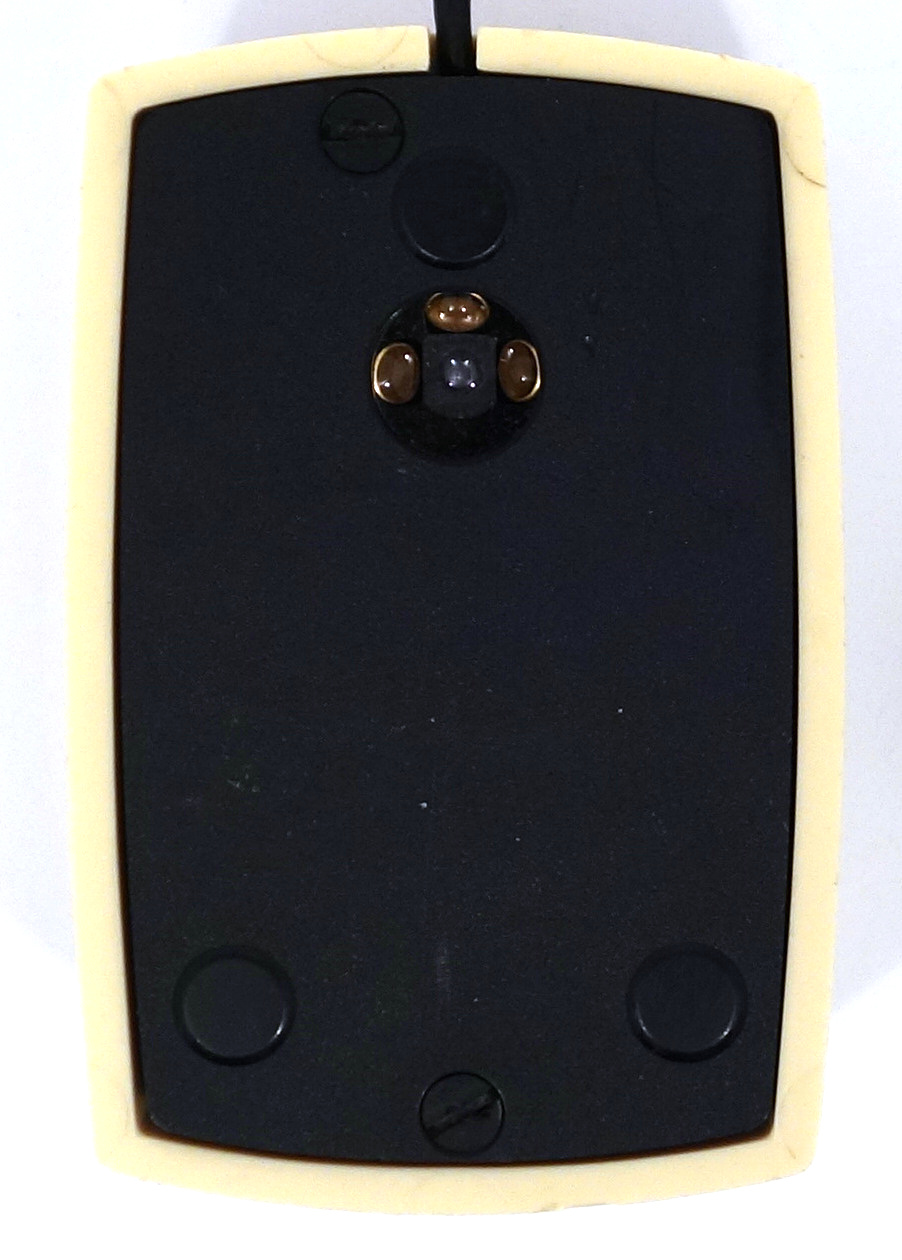
\includegraphics[scale=0.5]{1981_xerox_alto_mouse/bottom_30.jpg}
    \caption{Xerox Alto Optical Mouse, top and bottom views}
    \label{XeroxAltoTopAndBottom}
\end{figure}

A $4 \times 4$ size scanning elements matrix is responsible for reading color inhomogeneities at move, so the mouse required either a pad with a specially designed pattern or any surface with similar alternating light and dark spots, such as denim. The Xerox Alto optical mouse pad was a paper, sold in packs of 25 sheets \cite{pad}. The pattern was an array of light hexagons on a dark field and was easily reproduced by photocopying. A reconstructed pad can be seen in fig. \ref{fig:XeroxAltoPad}.

\begin{figure}[h]
    \centering
    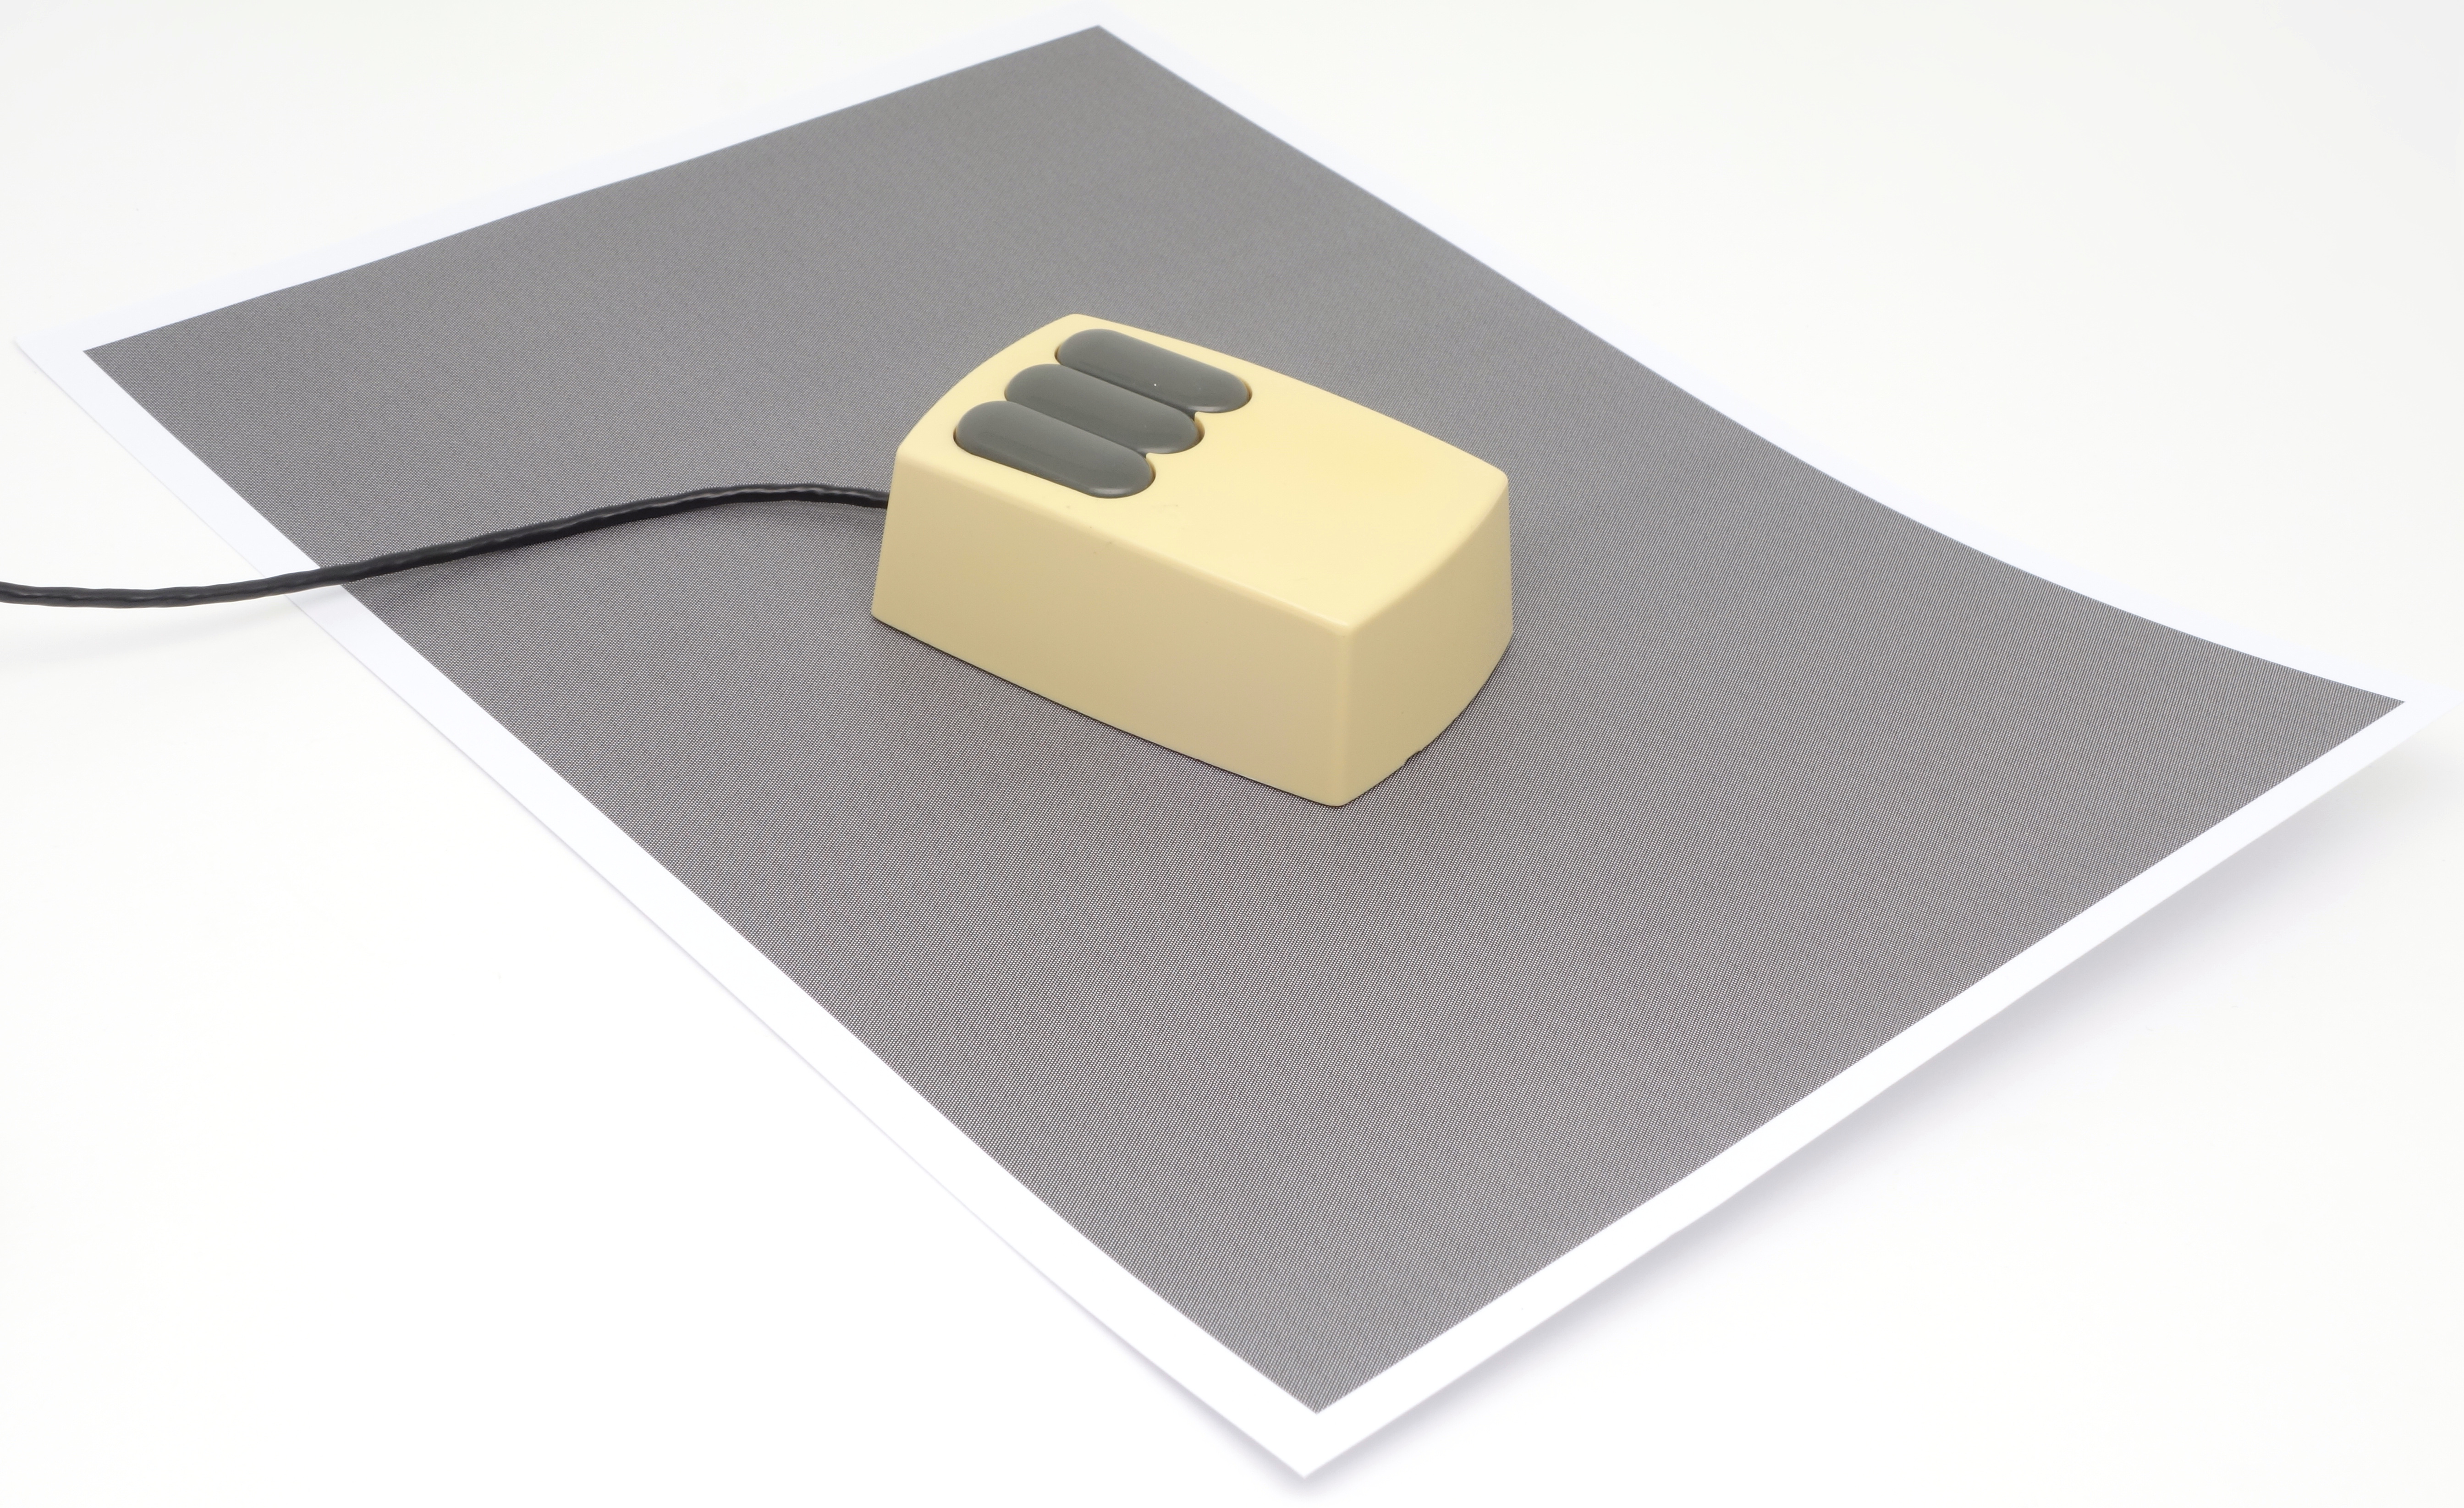
\includegraphics[scale=0.3]{1981_xerox_alto_mouse/pad_30.jpg}
    \caption{Xerox Alto Optical Mouse on a reconstructed pad}
    \label{fig:XeroxAltoPad}
\end{figure}

The mouse could have been smaller and lower in size if it had not used the standard Alto mouse body. As it is, it has the typical dimensions for mechanical mice of the first half of the 80s (figure \ref{fig:XeroxAltoSize}).

\begin{figure}[h]
    \centering
    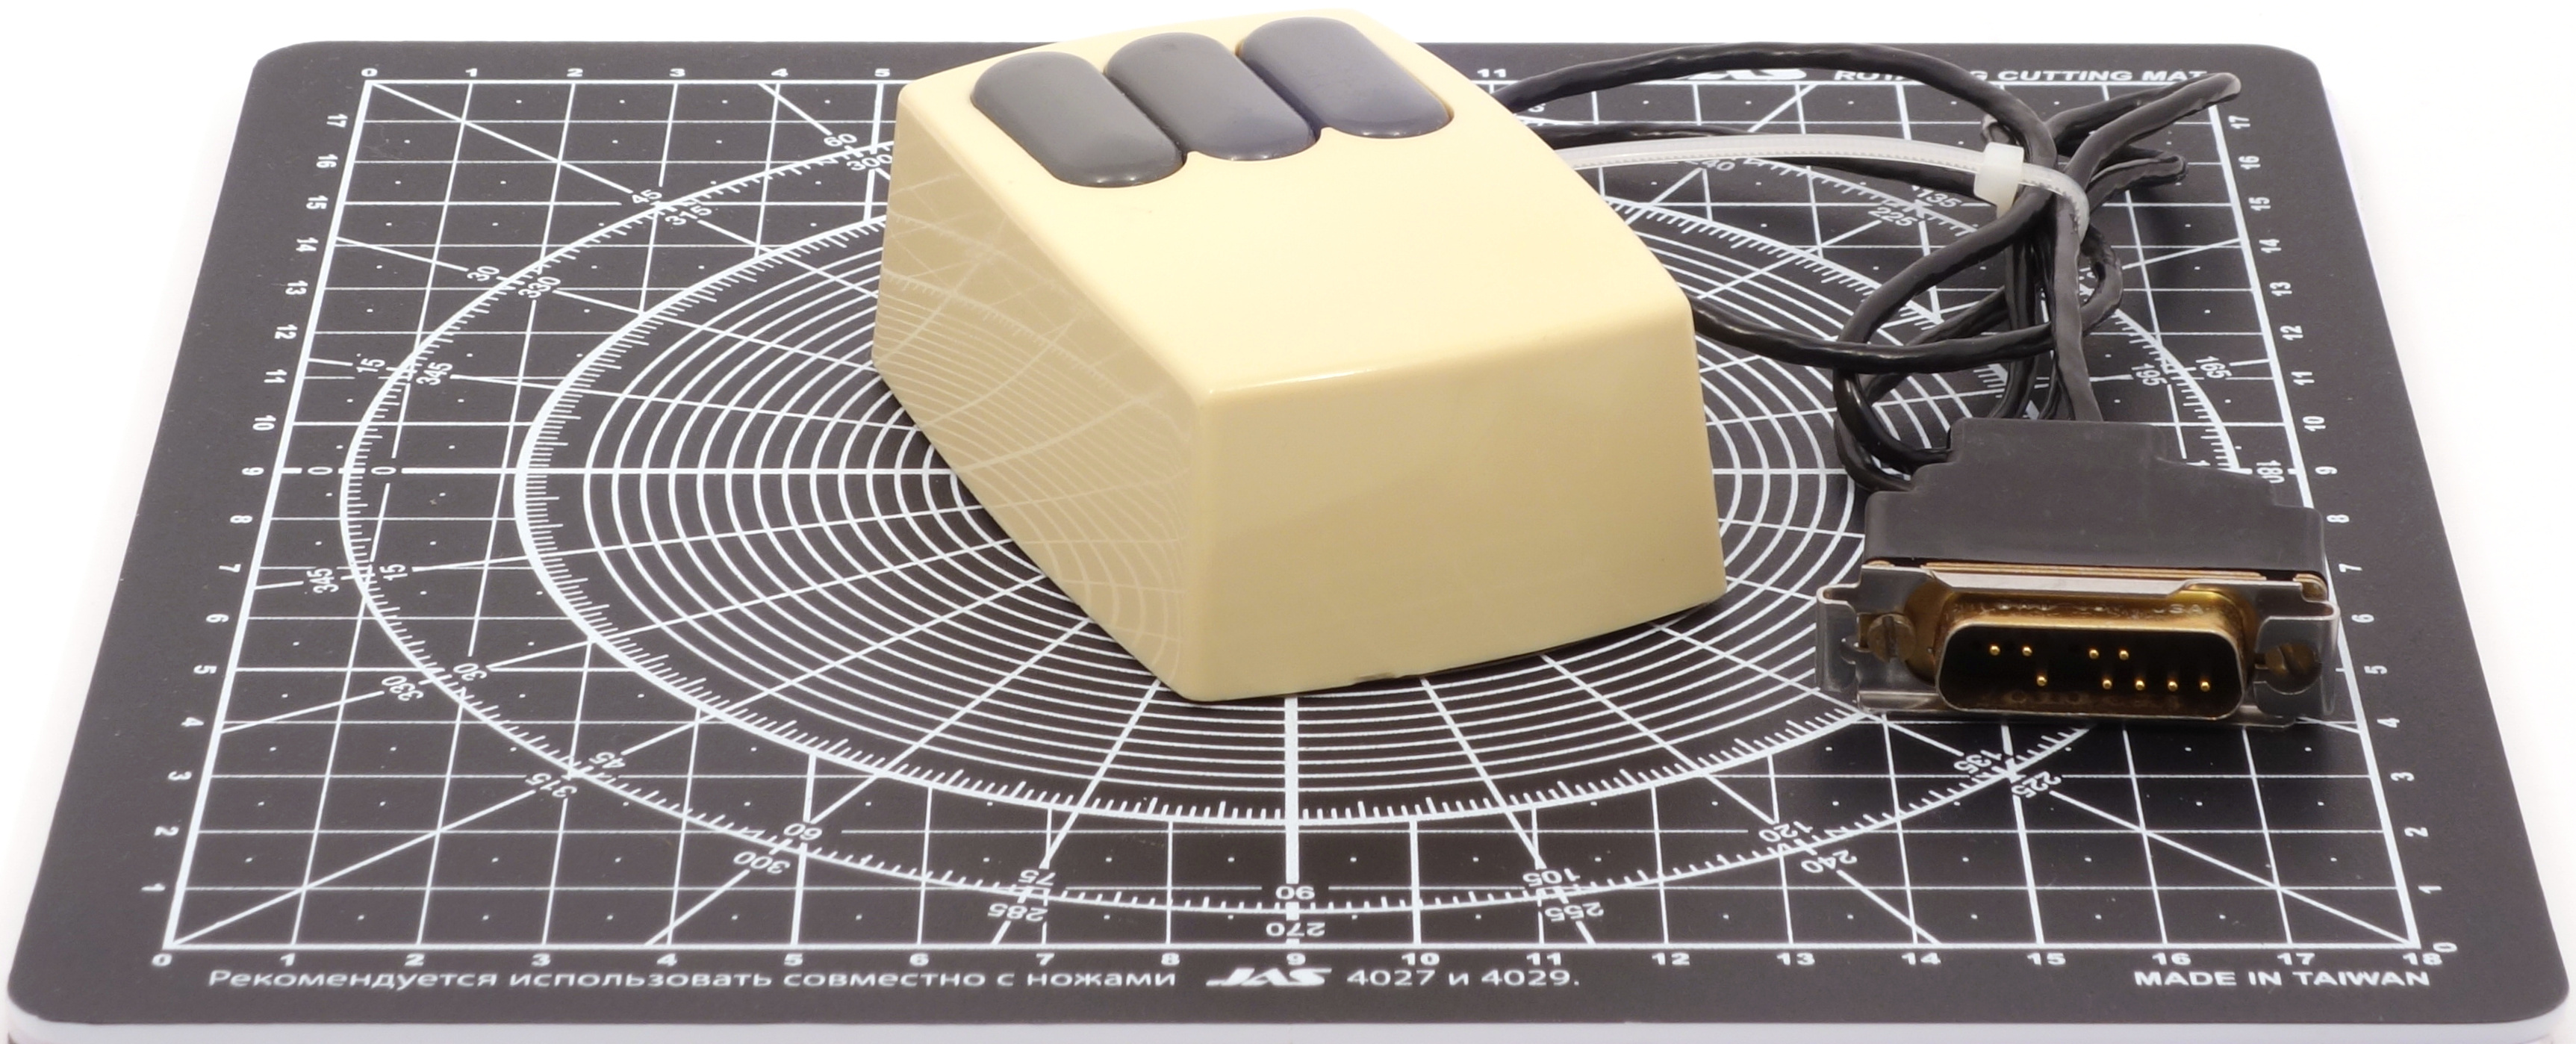
\includegraphics[scale=0.4]{1981_xerox_alto_mouse/size_15.jpg}
    \caption{Xerox Alto Optical Mouse on a graduated pad with a grid step of 1~cm}
    \label{fig:XeroxAltoSize}
\end{figure}

In terms of ergonomics and appearance, the Alto Mouse is minimalist. The user experience certainly suffers from the severe ``rectangularity'' of the case. Although this is partly compensated for by the convex oblong buttons, located within the reach of the fingers, the case doesn't provide much palm support (figure \ref{fig:XeroxAltoHand}).

\begin{figure}[h]
    \centering
    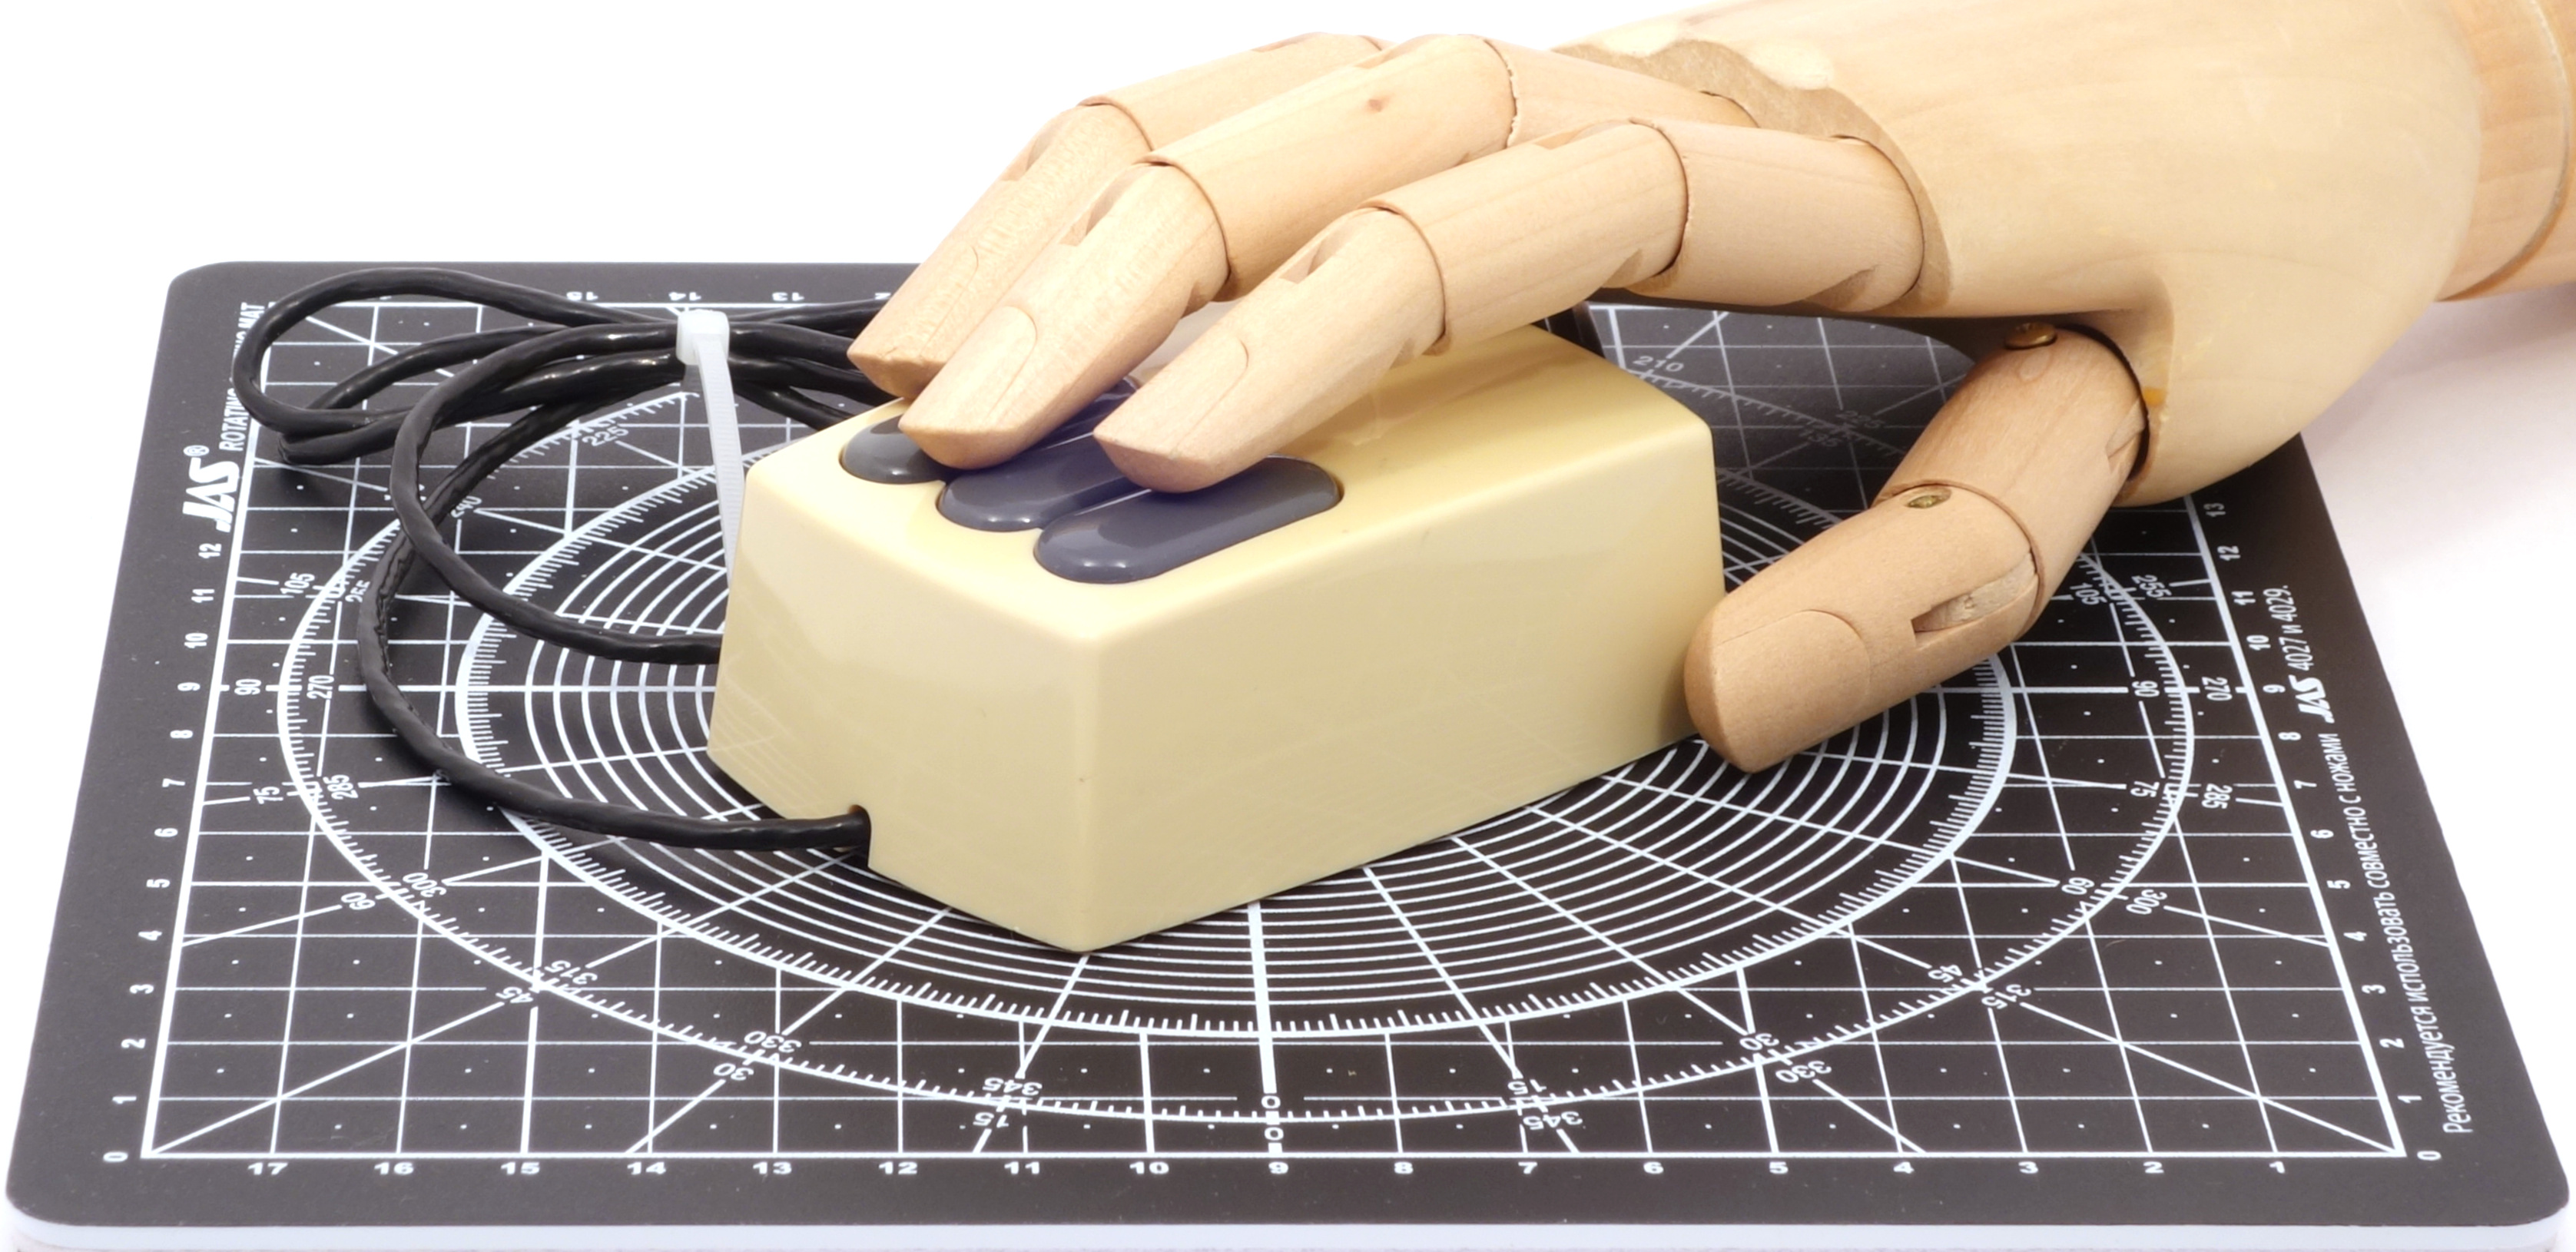
\includegraphics[scale=0.4]{1981_xerox_alto_mouse/hand_30.jpg}
    \caption{Xerox Alto Optical Mouse with a human hand model}
    \label{fig:XeroxAltoHand}
\end{figure}

The mouse has connector typical for Xerox Alto (DA-15 in this version), and the same quadrature interface as other Xerox mice. Mouse internals are shown in figure \ref{fig:XeroxAltoInside}, where you can see the plastic cover which protects the scanning matrix from possible exposure to light (in later versions of mice for the Xerox Star, this cover was removed), as well as the signal processing chip. The printed circuit board is raised above the base, and angle-directed LEDs placed under are illuminating the mouse pad.

\begin{figure}[h]
    \centering
    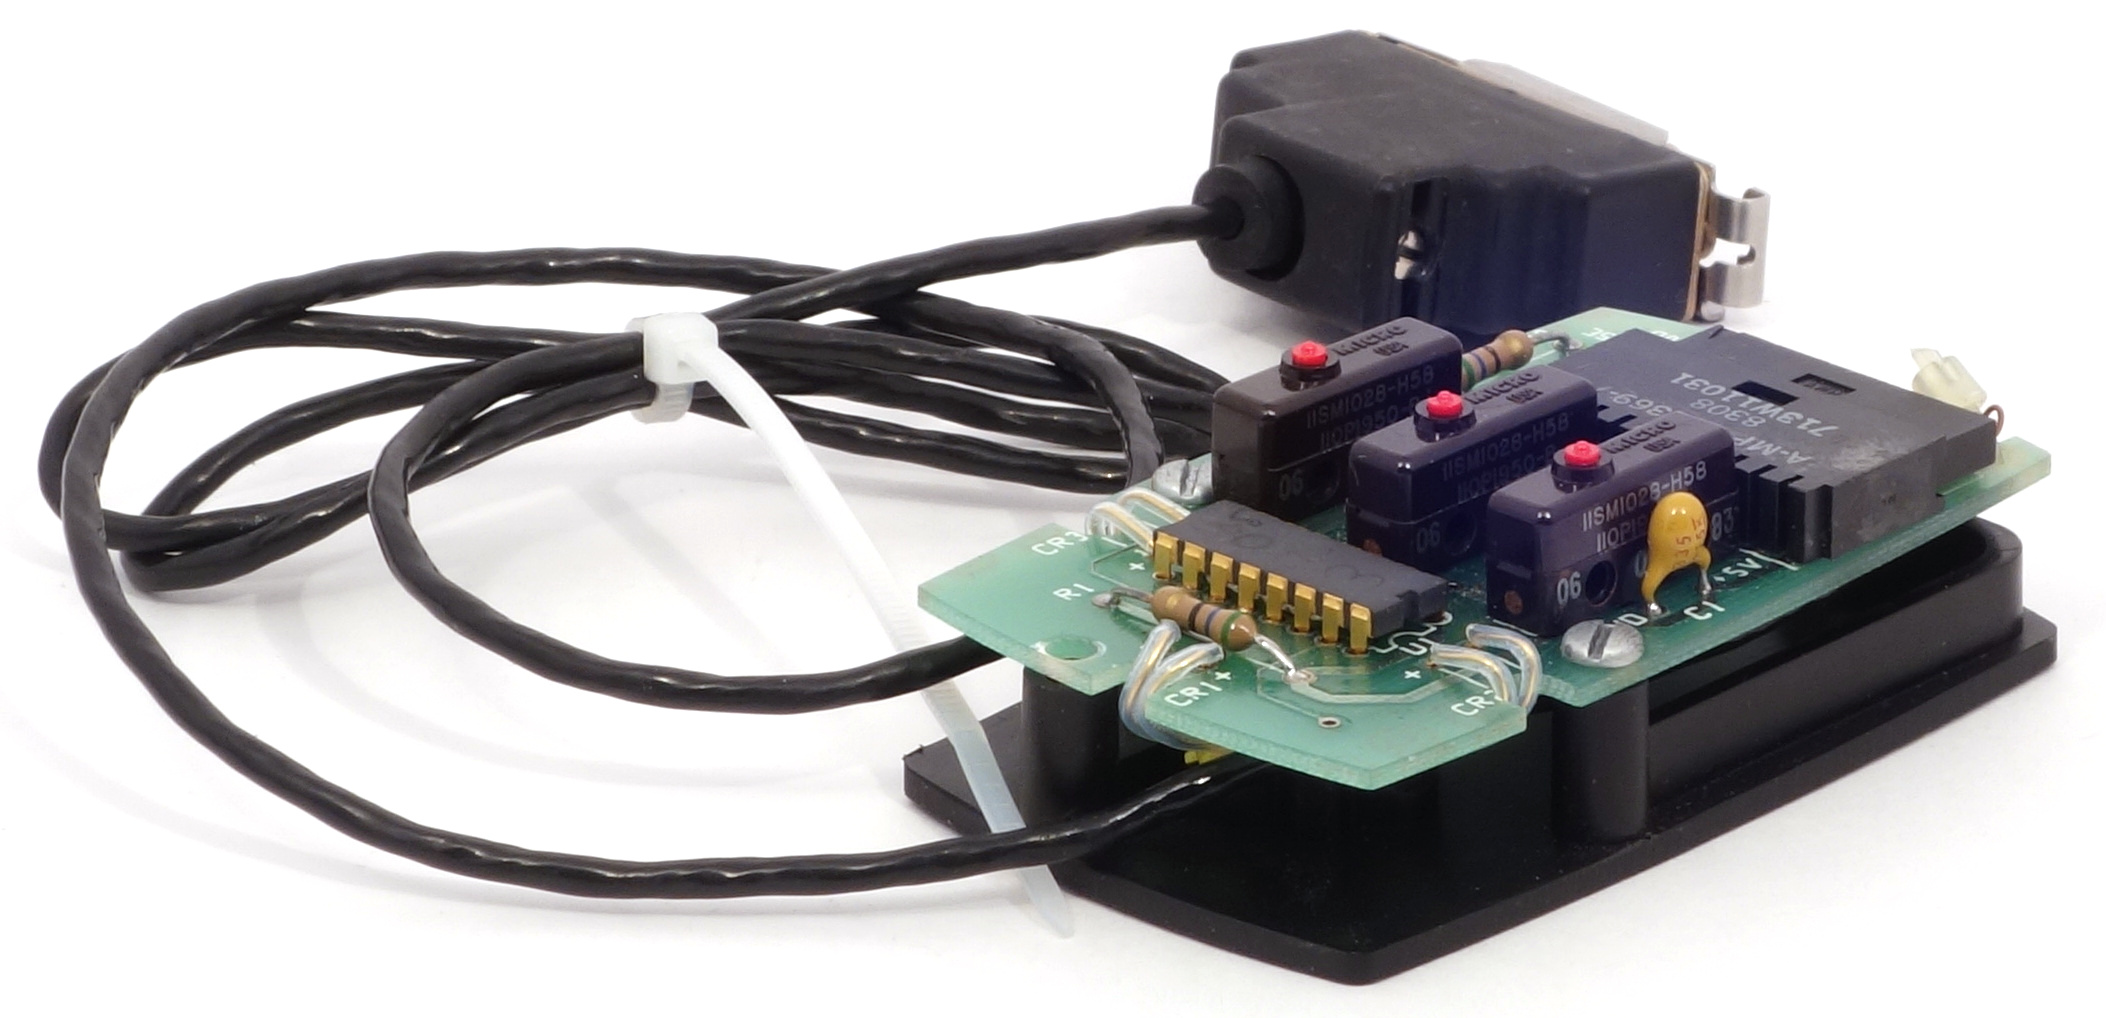
\includegraphics[scale=0.8]{1981_xerox_alto_mouse/inside_60.jpg}
    \caption{Xerox Alto Optical Mouse disassembled}
    \label{fig:XeroxAltoInside}
\end{figure}

\begin{thebibliography}{9}
\bibitem {wiki} Xerox Alto: Wikipedia \url{https://en.wikipedia.org/wiki/Xerox_Alto}
\bibitem {vlsi81} R.\,F. Lyon. The Optical Mouse, and an Architectural Methodology for
Smart Digital Sensors // VLSI DESIGN, August 1981. - p. 20--30. \url{https://www.dicklyon.com/tech/OMouse/OpticalMouse-Lyon.pdf}
\bibitem {vlsi82} R.\,F. Lyon, M.\,P. Haeberli. Designing and Testing The Optical Mouse // VLSI DESIGN, January/February, 1982. - p. 20--30. \url{https://www.dicklyon.com/tech/OMouse/DesigningTestingOMouse.pdf}
\bibitem{pad} R.\,F. Lyon The Optical Mouse: Early Biomimetic Embedded Vision / Advances in Embedded Computer Vision, Nov 2014, pp.3-22 \url{https://static.googleusercontent.com/media/research.google.com/ru//pubs/archive/43260.pdf}
\bibitem{mouses} Xerox Mice. oldmouse.com \url{https://web.archive.org/web/20210418000634/http://oldmouse.com/mouse/xerox/alto.shtml}
\end{thebibliography}
\end{document}
